\section*{Chapter 3. Evaluation of the proposed method}
\addcontentsline{toc}{section}{Chapter 3. Evaluation of the proposed method}
\setcounter{section}{3}
\setcounter{subsection}{0}
To assess the feasibility of the \ourmethodshort{}, comprehensive evaluation of the proposed solution has been applied with detailed results being presented in the article \cite{Demidovskij2025}. 

\subsection{Software implementation}
    The software implementation is made in a form of Python package, adhering to the principles of object-oriented programming, and is fully compatible with all the considered \llms{}. The code is the intellectual property of Huawei and cannot be disclosed in this work.

\subsection{Protocol}\label{subsec:protocol}
For the evaluation purposes, six \llms{} with different numbers of parameters were chosen to estimate the performance on different scales of \llms{}: 
\begin{itemize}
    \item \gpt{} (24 Transformer blocks);
    \item \llamaTwoSmall{} (32 Transformer blocks);
    \item \llamaTwoBig{} (40 Transformer blocks);
    \item \qwenSmall{} (36 Transformer blocks);
    \item \qwenMedium{} (28 Transformer blocks);
    \item \qwenLarge{} (64 Transformer blocks).
\end{itemize}
The \gpt{} model was taken from \textit{transformers v4.33.2},  \llamaTwoSmall{}, \llamaTwoBig{}, \qwenSmall{}, \qwenMedium{}, \qwenLarge{} models were taken from HuggingFace hub \cite{huggingface:llama2-7b}, \cite{huggingface:llama2-13b}, \cite{huggingface:qwen-small}, \cite{huggingface:qwen-medium}, \cite{huggingface:qwen-large}.

\begin{table}[H]
    \caption{Training hardware used for the evaluation of considered approaches.}
    \centering 
    \scriptsize
    \begin{tabularx}{0.99\textwidth}{M|x|x}
    \toprule
    & 
    \bfseries \gpt{} & 
    \bfseries \llamaTwoSmall{}, \llamaTwoBig{}, \qwenSmall{}, \qwenMedium{}, \qwenLarge{} \\
    \midrule
    % \bottomrule
    CPU & CPU 32 cores with 3.0GHz & CPU 32 cores with 2.90GHz \\ 
    \midrule
    OS & Ubuntu 20.04.6 LTS & Ubuntu 20.04.04 LTS \\
    \midrule
    Driver Version & 515.43.04 & 535.183.01 \\
    \midrule
    Kernel Version & 5.4.0-176-generic & 5.15.0-125-generic \\
    \midrule
    CUDA Toolkit Version & 11.7.64 & 12.2 \\
    \midrule
    Training Libraries & \textit{transformers} 4.33.0,  \textit{PyTorch} 2.1.0, \textit{DeepSpeed} 0.15.4, \textit{peft} v.0.18.0 & \textit{transformers} 4.45.0,  \textit{PyTorch} 2.1.0, \textit{DeepSpeed} 0.15.4, \textit{peft} v.0.18.0 \\
    \bottomrule
\end{tabularx}
\label{tab:hardware}
\end{table}

\begin{table}[H]
    \caption{Training protocol used for the evaluation of considered approaches.}
    \centering 
    \footnotesize
    \renewcommand{\arraystretch}{0.5}
    \begin{tabularx}{0.99\textwidth}{M|x|x}
    \toprule
    & 
    \bfseries \gpt{} & 
    \bfseries \llamaTwoSmall{}, \llamaTwoBig{}, \qwenSmall{}, \qwenMedium{}, \qwenLarge{} \\
    \midrule
    Sequence Length & 512 & 256 \\ 
    \midrule
    Learning Rate & 6e-4 & 1e-5 \\
    \midrule
    AdamW $\beta_1$ & 0.9 & 0.9 \\
    \midrule
    AdamW $\beta_2$ & 0.99 & 0.99 \\
    \midrule
    Weight Decay & 0.01 & 0 \\
    \midrule
    Epochs & 2 & 2 \\
    \midrule
    Precision & fp16 & bf16 \\
    \midrule
    \lora{} $r$ & 16 & 16 \\
    \midrule
    \lora{} $\alpha$ & 32 &  32\\
    \midrule
    Ratio of Transformer blocks & 0.8 &  0.6\\
    \bottomrule
\end{tabularx}
\label{tab:training_protocol}
\end{table}

Since \lora{} is the de-facto standard approach for fine-tuning acceleration, it was selected as a baseline for computational experiments on quality and acceleration. In addition, the most prominent modifications of \lora{}, such as \dora{} \cite{dora}, \pissa{} \cite{pissa}, \adalora{} \cite{adalora} were chosen as reference methods during the evaluation. The implementation of these approaches was taken from the \textit{peft v.0.18.0} library \cite{peft}.

Used training hardware and software are described in Table \ref{tab:hardware}. Training protocol for each model is described in Table \ref{tab:training_protocol}. The \textit{Ratio of Transformer blocks} row means the ratio of Transformer blocks selected for fine-tuning with chosen approaches. Notably, the \gpt{} model requires a higher number of updated layers than all other models, because a greater number of layers in the model allows for a smaller amount of updated layers, since a substantial proportion of the layers will still be updated.

After the fine-tuning, in order to estimate the final quality of the model, zero-shot accuracy was measured on commonsense reasoning datasets: PIQA \cite{piqa}, HellaSwag \cite{hellaswag}, Winogrande \cite{winogrande}, ARC \cite{arc}, OpenbookQA \cite{openbookqa}, MMLU \cite{mmlu} using the lm-evaluation-harness package \cite{lm_eval}. Zero-shot PPL was measured on language modelling dataset WikiText2 \cite{wikitext}. In this work, an average accuracy and perplexity are presented. The detailed results for each of these datasets are presented in the paper \cite{Demidovskij2025}.
\begin{table}[!t]
    \caption{Quality results after the fine-tuning with considered approaches on \gpt{}, \llamaTwoSmall{}, and \llamaTwoBig{}.}
    \centering  
    \scriptsize
    \begin{tabularx}{0.99\textwidth}{AM|TTT}

        \toprule

        \bfseries Model &
        \bfseries Method & 
        \bfseries Average accuracy, \(\uparrow\) & 
        \bfseries Perplexity, \(\downarrow\) &
        \bfseries Acceleration, \(\uparrow\) \\

        \midrule 
        \multirow{11}{*}{\gpt{}}
        & \lora{} (baseline) & 37.5 & 173.1 & -- \\
        \cmidrule{2-5}
        & \dora{} & 37.0 & 184.2 & -21.6 \\
        & \pissa{} & 34.9 & 172.1 & 0.9 \\
        & \adalora{} & 36.9 & 179.2 & -1.3 \\
        \cmidrule{2-5}
        & \uidl{} & 37.9 & 173.8 & -39.5 \\
        & \lisa{} & \bfseries 40.8 & 205.7 & -40.9 \\
        & \ows{} & 31.3 & 180.2 & -61.3 \\
        & \sleb{} & 36.3 & 450.1 & 13.5 \\
        & \shortllama{} & 33.1 & 400.5 & 12.6 \\
        \cmidrule{2-5}
        & \cellcolor{DarkOliveGreen3} \ourmethodshort{} & \cellcolor{DarkOliveGreen3} 38.0 & \cellcolor{DarkOliveGreen3} \bfseries 72.7 & \cellcolor{DarkOliveGreen3} \bfseries 25.2 \\
        \midrule
        \multirow{9}{*}{\llamaTwoSmall{}}
        & \lora{} (baseline) & 59.9 & \bfseries 9.2 & -- \\
        \cmidrule{2-5}
        & \dora{} & 59.8 & \bfseries 9.2 & -407.3 \\
        & \pissa{} & \bfseries 60.9 & 9.4 & 1.7 \\
        & \adalora{} & 59.3 & \bfseries 9.2 & -51.6 \\
        \cmidrule{2-5}
        & \uidl{} & 59.3 & \bfseries 9.2 & -31.2 \\
        & \sleb{} & 42.7 & 403.6 & -11.0 \\
        & \shortllama{} & 41.1 & 53.1 & 13.4 \\
        \cmidrule{2-5}
        & \cellcolor{DarkOliveGreen3} \ourmethodshort{} & \cellcolor{DarkOliveGreen3} 59.4 & \cellcolor{DarkOliveGreen3} \bfseries 9.2 & \cellcolor{DarkOliveGreen3} \bfseries 29.2 \\
        \midrule
        \multirow{9}{*}{\llamaTwoBig{}}
        & \lora{} (baseline) & 63.8 & \bfseries 7.7 & -- \\
        \cmidrule{2-5}
        & \dora{} & 63.7 & \bfseries 7.7 & -203.3 \\
        & \pissa{} & \bfseries 64.5 & 7.9 & -0.3 \\
        & \adalora{} & 63.1 & \bfseries 7.7 & -92.9 \\
        \cmidrule{2-5}
        & \uidl{} & 63.6 & \bfseries 7.7 & -22.7 \\
        & \sleb{} & 49.8 & 20.0 & -70.0 \\
        & \shortllama{} & 42.4 & 72.8 & -110.7 \\
        \cmidrule{2-5}
        & \cellcolor{DarkOliveGreen3} \ourmethodshort{} & \cellcolor{DarkOliveGreen3} 63.6 & \cellcolor{DarkOliveGreen3} \bfseries 7.7 & \cellcolor{DarkOliveGreen3} \bfseries 44.8 \\
        \midrule
        \multirow{9}{*}{\qwenSmall{}}
        & \lora{} (baseline) & 62.9 & 15.5 & -- \\
        \cmidrule{2-5}
        & \dora{} & 62.9 & 15.3 & -201.0 \\
        & \pissa{} & \bfseries 63.5 & \bfseries 11.8 & -0.6 \\
        & \adalora{} & 62.3 & 15.1 & -71.5 \\
        \cmidrule{2-5}
        & \uidl{} & 62.7 & 15.5 & -20.1 \\
        & \sleb{} & 44.5 & 77.4 & -30.4 \\
        & \shortllama{} & 15.1 & 72.8 & 0.1 \\
        \cmidrule{2-5}
        & \cellcolor{DarkOliveGreen3} \ourmethodshort{} & \cellcolor{DarkOliveGreen3} 62.9 & \cellcolor{DarkOliveGreen3} 15.5 & \cellcolor{DarkOliveGreen3} \bfseries 28.6 \\
        \midrule
    \end{tabularx}
    \label{tab:quality_1}
\end{table}
\subsection{Analysis of the obtained results}
Computational experiments with chosen models and approaches are presented in Table \ref{tab:quality_1}. For \qwenLarge{} model, the evaluation of \dora{} approach was not presented, as memory requirements did not fit to used hardware.

\ourmethodshort{} provides an average acceleration of 33.1\%
with a considerable maximum speedup of 44.8\% for \llamaTwoBig{}
with a quality decrease of less than 0.2\%.  In addition, \ourmethodshort{} significantly outperforms \pissa{}, \dora{}, and \adalora{} from the point of acceleration, and provides 0.4\% of quality improvement compared to \textit{\adalora{}} and comparable performance to \textit{\dora{}}. However, it leads 0.2\% quality decrease compared to \pissa{} as \pissa{} employs an SVD initialization
of \lora{} \(A, B\) adapters, which provides them with the most important information from the original weights \(W\).

\subsection{Sensitivity analysis}
    Sensitivity analysis of \(\alpha\) and \(h\) hyperparameters of \ourmethodshort{} and importance metrics is presented in Figure \ref{fig:ablation_alpha}, Figure \ref{fig:ablation_h}, and Figure \ref{fig:ablation_importance}. They were analyzed in terms of their impact on the resulting quality and acceleration.
    \subsubsection{Analysis of hyperparameter \(\alpha\)}
        \begin{figure}[H]
            \centering
            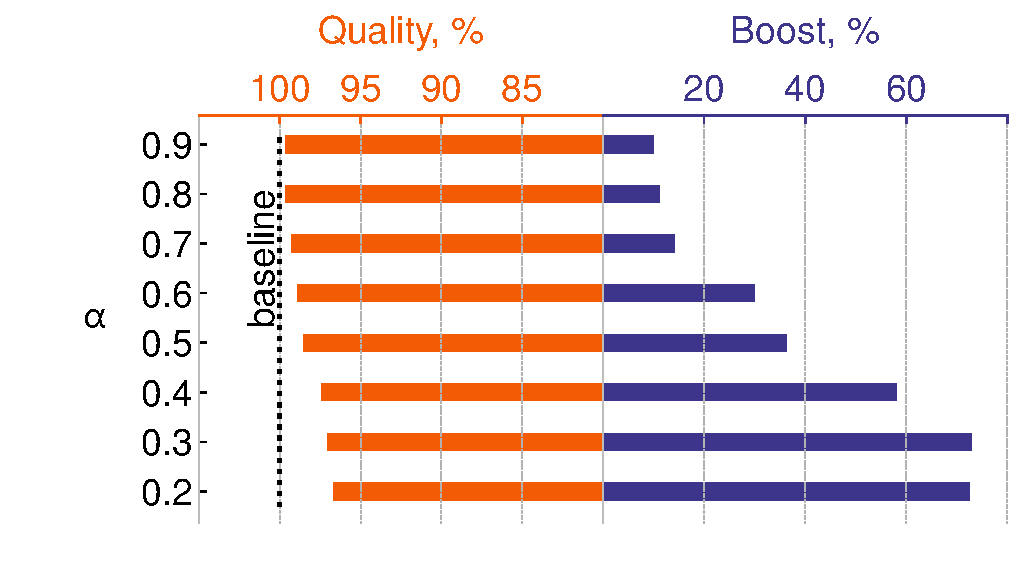
\includegraphics[width=0.6\textwidth]{sections/figures/ablation_alpha.pdf}
            \caption{Sensitivity analysis of \ourmethodshort{} to the \(\alpha\) hyperparameter. \(h\) is 10, importance metric is cosine similarity.}
            \label{fig:ablation_alpha}
        \end{figure}
        Ablation study of the \(\alpha\) hyperparameter of
        \ourmethodshort{} is presented in Figure \ref{fig:ablation_alpha}. Obtained results demonstrate that increasing \(\alpha\) significantly affects both acceleration and model quality. In particular, a maximum speedup of 72.6\% is observed at \(\alpha\) = 0.2, where only 20\% of the Transformer blocks are trained. However, it leads to a 3.3\% increase in perplexity, suggesting underfitting. Minimal quality degradation (0.3\%) occurs at higher \(\alpha\) values (0.8 and 0.9), where 80-90\% of the Transformer blocks are trained initially. \(\alpha\) = 0.6 is identified as the optimal setting for balancing speed and quality. 
    \subsubsection{Analysis of hyperparameter \(h\)}
        \begin{figure}[H]
            \centering
            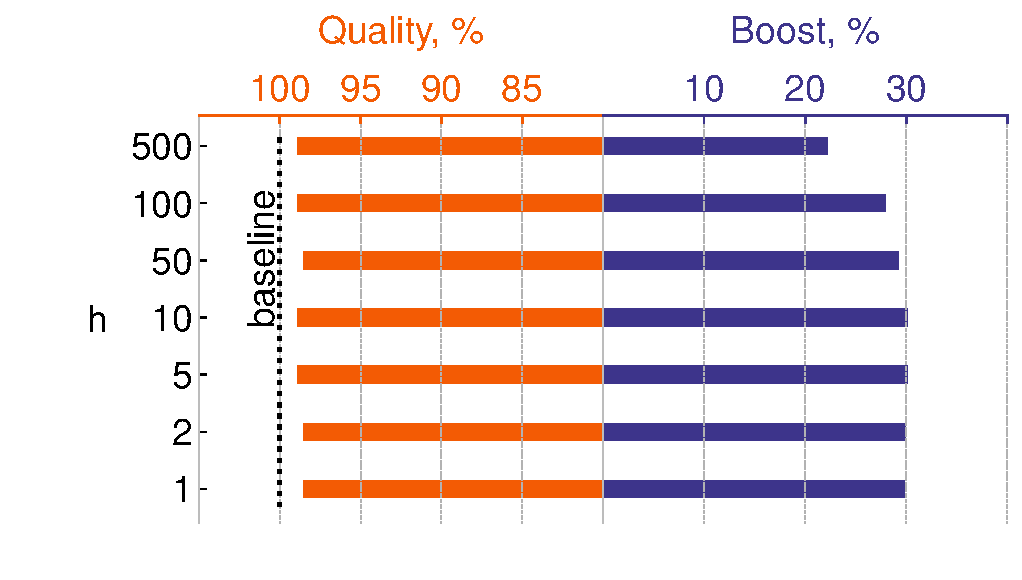
\includegraphics[width=0.6\textwidth]{sections/figures/ablation_h.pdf}
            \caption{Sensitivity analysis of \ourmethodshort{} to the \(h\) hyperparameter. \(\alpha\) is 0.6, importance metric is cosine similarity.}
            \label{fig:ablation_h}
        \end{figure}
        Ablation study of the \(h\) hyperparameter of
        \ourmethodshort{} is presented in Figure \ref{fig:ablation_h}. According to the achieved results, variations in hyperparameter \(h\) do not significantly impact quality, with only a 0.3\% change in perplexity was observed between \(h\) = 1 and \(h\) = 500. The smallest \(h\) value accelerates fine-tuning by 29.8\%, indicating that even a single training step can adequately capture the importance of a Transformer block. This observation is supported by the relative stability of model quality across different \(h\) settings, as shown in Figure \ref{fig:ablation_h}. \(h\) = 10 is identified as the optimal setting for balancing speed and quality. 
    \subsubsection{Analysis of importance metrics}
        \begin{figure}[H]
            \centering
            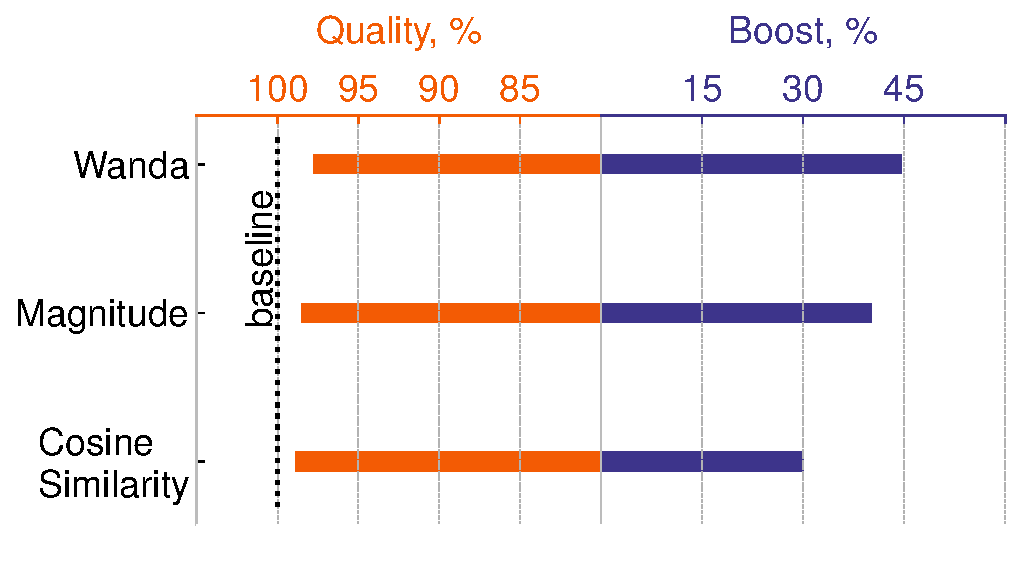
\includegraphics[width=0.6\textwidth]{sections/figures/ablation_importance.pdf}
            \caption{Sensitivity analysis of \ourmethodshort{} to considered importance metrics. \(\alpha\) is 0.6, \(h\) is 10.}
            \label{fig:ablation_importance}
        \end{figure}
         An ablation study of importance metrics is presented in Figure \ref{fig:ablation_importance}. 
         Despite the fact, that cosine similarity is considered an optimal choice, an additional ablation study on applying standard pruning metrics, such as Magnitude (\ref{eq:magnitude}) and Wanda (\(\ref{eq:wanda}\)) was performed. Notably, Magnitude and Wanda importance metrics are adapted to Transformer block importance estimation as described in Definition \ref{def:transformer-block-importance}.
        \begin{definition}\label{def:transformer-block-importance}
            Let \(T\) denote Transformer blocks, \(i_{\xi}\) denote importance score for \(\xi\) layer inside it, then importance of Transformer block is defined as:
            \begin{equation}\label{eq:aggregation}
                I(T) = \frac{\sum_{\xi \in T} i_{\xi}}{|T|}
            \end{equation}
        \end{definition}
        Sensitivity analysis reveals that the Magnitude metric yields the best balance between acceleration and quality. In contrast, the Wanda metric, despite considering input activations, provides a higher speedup at the
        cost of increased quality degradation by 2\% compared to the baseline. Although cosine similarity decelerates the fine-tuning on 7\% compared with the Magnitude, it degrades model quality the least, representing the most suitable choice, as minimizing the drop in model quality is particularly crucial in the context of importance-based fine-tuning. This conclusion is also consistent with the results of last year's study.
    \subsection{Summary}
        In conclusion, the quality and acceleration of the proposed \ourmethodshort{} was estimated across different \llm{} scales (350M, 3B, 7B, 13B, 32B) and a broad range of tasks. According to the obtained results, \ourmethodshort{} significantly outperforms the baseline \lora{} approach and reference \dora{}, \pissa{}, and \adalora{} methods from the point of acceleration. \ourmethodshort{} provides on average 33\% of fine-tuning time speedup compared to \lora{} approach. Moreover, \ourmethodshort{} achieves near-lossless performance with an average quality degradation of 0.2\% compared to baseline \lora{} approach. 
        
        According to the conducted ablation study, the hyperparameter \(\alpha=0.6\) and hyperparameter \(h=10\) are considered an optimal choice with importance metric being cosine similarity. 
